%% -*- TeX-master: t -*-

%% \documentclass{acm_proc_article-sp}
\documentclass{sig-alternate}


%%%%%%%%%%%%%%%%%%%%%%%%%%%%%%%%%%%%%%%%%%%%%%%%%%%%%%%%%%%%%%%%%%%%%%%%
%%
%% standard texmf packages
%%

\usepackage{amsmath}
\usepackage{ifthen}
\usepackage{nicefrac}
\usepackage{fancyvrb}
\usepackage{subfigure}
\usepackage{xspace}

\usepackage[bookmarks, pdftitle={Bug Isolation in the Presence of
  Multiple Errors}, pdfauthor={Ben Liblit, Mayur Naik, Alice X.
  Zheng, Alex Aiken, and Michael I.  Jordan}, pdfsubject={D.2.4
  [Software Engineering]: Software/Program Verification -- statistical
  methods; D.2.5 [Software Engineering]: Testing and Debugging --
  debugging aids, distributed debugging, monitors, tracing; I.5.2
  [Pattern Recognition]: Design Methodology -- feature evaluation and
  selection}, pdfkeywords={bug isolation, random sampling, invariants,
  feature selection, statistical debugging},
pdfpagemode=UseOutlines]{hyperref}

\ifthenelse{\isundefined{\pdfoutput}}{}{\usepackage{thumbpdf}}


%%%%%%%%%%%%%%%%%%%%%%%%%%%%%%%%%%%%%%%%%%%%%%%%%%%%%%%%%%%%%%%%%%%%%%%%
%%
%% unique to this paper
%%

\usepackage{Autoref}
\newcommand{\subfigureautorefname}[0]{Figure}

%% assorted handy macros
\newcommand{\moss}{\textsc{Moss}\xspace}
\newcommand{\termdef}[1]{\textit{#1}}
\newcommand{\prob}{\mbox{\textit{Prob}}}
\newcommand{\fail}{\mbox{\textit{Fail}}}
\newcommand{\crash}{\mbox{\textit{Crash}}}
\newcommand{\context}{\mbox{\textit{Context}}}
\newcommand{\increase}{\mbox{\textit{Increase}}}
\renewcommand{\H}{{\mathcal{H}}}


%%%%%%%%%%%%%%%%%%%%%%%%%%%%%%%%%%%%%%%%%%%%%%%%%%%%%%%%%%%%%%%%%%%%%%%%
%%
%% front matter
%%

\title{Bug Isolation in the Presence of Multiple Errors
  %%
  \thanks{This research was supported in part by NASA Grant No.\
    NAG2-1210; NSF Grant Nos.\ EIA-9802069, CCR-0085949, ACI-9619020,
    and IIS-9988642; DOE Prime Contract No.\ W-7405-ENG-48 through
    Memorandum Agreement No.\ B504962 with LLNL; and ONR MURI
    N00014-00-1-0637.  The information
    presented here does not necessarily reflect the position or the
    policy of the Government and no official endorsement should be
    inferred.}}

\numberofauthors{3}

\makeatletter
\newcommand*{\eecsMark}[0]{\@fnsymbol{2}}
\newcommand*{\statMark}[0]{\@fnsymbol{3}}
\newcommand*{\stanMark}[0]{\@fnsymbol{4}}
\makeatother
\newcommand*{\eecs}[0]{\textsuperscript{\eecsMark}}
\newcommand*{\stat}[0]{\textsuperscript{\statMark}}
\newcommand*{\both}[0]{\textsuperscript{\eecsMark, \statMark}}
\newcommand*{\stan}[0]{\textsuperscript{\stanMark}}

\newcommand{\moreauthors}[0]{\end{tabular}\\\vspace{-.5\baselineskip}\begin{tabular}{c}}

\author{
  \alignauthor Ben Liblit \eecs \\
  \alignauthor Mayur Naik \stan \\
  \alignauthor Alice X.\ Zheng \eecs \\
  \moreauthors
  \global\multiply\auwidth by 3
  \global\divide\auwidth by 2
  \alignauthor Alex Aiken \stan \\
  \alignauthor Michael I.\ Jordan \both
  \moreauthors
  \alignauthor
  \affaddr{\eecs Department of Electrical \\ Engineering and Computer Science} \\
  \affaddr{\stat Department of Statistics} \\
  \affaddr{University of California, Berkeley} \\
  \affaddr{Berkeley, CA 94720-1776}
  \alignauthor
  \affaddr{\stan Computer Science Department} \\
  \affaddr{353 Serra Mall} \\
  \affaddr{Stanford University} \\
  \affaddr{Stanford CA 94305-9025}
}

\bibliographystyle{abbrv}


%%%%%%%%%%%%%%%%%%%%%%%%%%%%%%%%%%%%%%%%%%%%%%%%%%%%%%%%%%%%%%%%%%%%%%%%
%%
%%  document body
%%

\begin{document}

\conferenceinfo{PLDI'04,}{June 9--11, 2004, Washington, DC, USA.}
\CopyrightYear{2004}
%% \crdata{}
\maketitle

\begin{abstract}
  Software errors are a fact of life, with complex programs exhibiting
  multiple bugs even within a single run.  Debugging can be difficult
  when neither the causes nor even the number of distinct errors are
  known.  We present a multiple-bug isolation algorithm that operates
  on sparsely sampled data drawn from large numbers of user runs.  By
  identifying those program behaviors which significantly increase the
  likelihood of failure, our technique helps guide software engineers
  to the most significant flaws in an application.  The approach has
  connections to statistical hypothesis testing, and is validated
  using a case study of a complex application.
\end{abstract}

\category{D.2.4}{Software Engineering}{Software/Program
  Verification}[statistical methods]
%%
\category{D.2.5}{Software Engineering}{Testing and
  Debugging}[debugging aids, distributed debugging, monitors, tracing]
%%
\category{I.5.2}{Pattern Recognition}{Design Methodology}[feature
  evaluation and selection]

\terms{Experimentation, Reliability}

\keywords{bug isolation, random sampling, invariants, feature
  selection, statistical debugging}


\section{Introduction}
\label{sec:introduction}

Programs are buggy.
%We all know this, and yet we use them anyway.
Most software ships with many known and unknown bugs; software
engineers understand that it is impractical to delay releasing code
until the last bug has been fixed.

Our vision is to use \termdef{statistical debugging} to
improve software quality.  Specially
instrumented programs monitor their own behavior and send feedback
reports to a central collection server.  Monitoring is both sparse and
random, so complete information is never available about
any single run.  However, monitoring is also lightweight and therefore
practical to deploy to user communities numbering in the thousands or
millions.  Statistical debugging does not seek to understand the
single cause of a single failure on one machine; rather, it identifies
broad statistical trends that isolate bug causes across many thousands
or millions of runs.  Because the process is driven by data from real
users, it implicitly attends to those program behaviors that cause the
most problems for the most users, most often.

In our previous work we examined the problem of automatically
isolating the cause of a single bug
\cite{PLDI`03*141,Zheng:2003:SDSP}.  As discussed above, however, no
realistic application has only a single bug, or even a handful of
bugs.  Consider the fact that the Mozilla web browser project has a
``topcrash'' software QA team specifically dedicated to identifying
and tracking the top forty most common crash bugs.  This cut-off is
not because anyone believes that there are only forty bugs; it is an
acknowledgment that engineering resources are finite so the most
important bugs should be fixed first.

This paper is about simultaneously isolating multiple bugs in complex
applications.  The main contributions are:

\begin{itemize}

\item We give a new algorithm for isolating multiple bugs
(\Autoref{sec:algorithm}).  Our algorithm is very efficient and works well in the
presence of multiple bugs, sparse sampling, and non-deterministic failure
modes.

\item We present a significant experimental study showing the
effectiveness of our algorithm on a complex application
(Sections~\ref{sec:experiments:setup}
and~\ref{sec:experiments:results}).  We seeded a program with nine
bugs, most
of which were taken directly from the application's bug log.  Our
system correctly identified a distinct cause for seven of the bugs; the
other two bugs never caused the program to fail in our experiment.
Our algorithm also discovered a new, previously unknown bug in the
application.

\end{itemize}

After providing some background on our previous work in single-bug
isolation (\Autoref{sec:background}), we discuss the algorithm (\Autoref{sec:algorithm}),
the design of our experiment (\Autoref{sec:experiments:setup}), and
the experimental results (\Autoref{sec:experiments:results}).
The paper winds up with a discussion of related work (\Autoref{sec:related-work})
and future work and conclusions (\Autoref{sec:conclusions}).

\section{Background}
\label{sec:background}

This section summarizes our previous work in isolating single bugs
\cite{PLDI`03*141,Zheng:2003:SDSP}, which is the starting point for
this work.  The ideal program monitoring system would gather complete
execution traces and provide them to an engineer (or, more likely, a
tool) to mine for the causes of bugs.  However, complete tracing of
program behavior is simply impractical; no end user would accept the
required performance overhead or network bandwidth.

Instead, we use a combination of sparse random sampling, which controls
performance overhead, and client-side summarization of the data, which
limits the storage and transmission costs.  We briefly discuss
both aspects.

Random sampling is added to a program via a source-to-source transformation.
Our sampling transformation is general: any collection of
statements within (or added to) a program may be designated as
``instrumentation'' and thereby sampled instead of run
unconditionally.  That is, each time instrumentation code is reached,
a coin flip decides whether the instrumentation is executed or not.
Coin flipping is simulated in a statistically fair
manner equivalent to a Bernoulli process: each potential sample is
taken or skipped randomly and independently as the program runs.
We have found that a sampling rate of \nicefrac{1}{100} keeps the performance overhead
of instrumentation low, often unmeasurable.

Orthogonal to the sampling transformation is the decision about what
instrumentation to introduce and how to concisely
summarize the resultant data.  This determines what behaviors one can
possibly observe once the sampling transformation is applied.  A useful instrumentation
scheme should be fairly general but selected to capture behaviors
which are likely to be of interest when hunting for bugs.  At present
our system offers the following instrumentation schemes:

\begin{description}
\sloppy
\item[branches:] At each conditional,
  count how often each branch is taken.  The observation is
  made just after the predicate is evaluated but before the selected
  branch is taken.  This scheme also applies to implicit conditionals
  in loops and logical operators (\texttt{\&\&}, \texttt{||},
  \texttt{?:}).  Each conditional induces one instrumentation site
  with two counters: number of times branched true and number of times
  branched false.

\item[returns:] In C, the
  sign of a return value is often used to encode an operation's success or failure.
  At each scalar-returning function call site, count how
  often the returned value is negative, zero, or positive.  For
  pointer-returning calls, this reduces to counting
  \texttt{NULL} versus non-\texttt{NULL}.  The observation is made
  just after the function returns but before the result is used by the
  original program.  An instrumentation site is added even if the
  source program discards the return value, as unchecked return
  values are a common source of bugs.  Each call site induces one
  instrumentation site with three counters: number of negative
  returns, number of zero returns, and number of positive returns.

\item[scalar-pairs:] Many bugs
  concern boundary issues exposed by the relationship between a pair
  of variables, or between a variable and some program constant.  At
  each scalar assignment \texttt{x = \dots}, identify each
  \emph{other} same-typed in-scope variable $\mathtt{y}_i$ and each
  constant expression $\mathtt{c}_j$.  Count how often the new value
  for \texttt{x} is less than, equal to, or greater than each
  $\mathtt{y}_i$ and each $\mathtt{c}_j$.  The observation is made
  after both sides of the assignment have been evaluated but
  before the assignment takes place.  This lets us compare
  \texttt{x} to \texttt{x} as well, effectively comparing the new and
  old values of the left-hand side.  Each compared-to $\mathtt{y}_i$
  or $\mathtt{c}_j$ is treated as a distinct instrumentation site;
  thus a single assignment may induce a large number of sites.  Each
  such site maintains three counters: how often the value being
  assigned is less than, equal to, or greater than the compared-to
  variable or constant.
\end{description}

The common theme among these instrumentation schemes is that we
instrument program predicates and count the number of times that these
predicates are observed to be true or false when a sample is taken.
For the returns and scalar-pairs instrumentation schemes, the three
predicates that are tracked explicitly actually give rise to a family
of six predicates that we use in our analysis of the data.
For example, for each scalar-pairs comparison between \texttt{x} and \texttt{y}, one and
only one of the three predicates $\mathtt{x} < \mathtt{y}$, $\mathtt{x} = \mathtt{y}$, or
$\mathtt{x} > \mathtt{y}$ can be true.  Thus one observation at one
site always updates exactly one of that site's counters.  An
observation that $\mathtt{x} < \mathtt{y}$ is true is therefore equivalent to
an observation that $\mathtt{x} \geq \mathtt{y}$ is false.  Similarly, we can
infer from the data the two remaining predicates $\mathtt{x} \leq \mathtt{y}$ or
$\mathtt{x} \neq \mathtt{y}$.

Also note that because some counter is always incremented at every
sample in all three schemes, we can easily determine the number of
times a site was sampled by summing all the counters for the site
(two counters for the branches instrumentation and three counters for
the others).  Thus, we can distinguish between predicates that are
never observed during execution (all the counters at the site are 0)
and predicates that are observed but never true (the counter(s) for the predicate
is 0, but some other counter at the site is positive).

The post-execution feedback report consists of the final counter values for
each instrumentation site.  Reducing a trace to a set of counters
prevents us from reasoning about relative time ordering of events
during execution.  However, it also means that program actions early
in execution remain just as visible as those much later.  This
contrasts with traditional postmortem debugging tools which expose
only the final state of the program at the point of failure.

\section{Cause Isolation Algorithm}
\label{sec:algorithm}
\placeholder{ We need to make sure we mention somewhere that (1) predicates are conceptually sampled after the line
is executed and (2) we transform our counters into real predicates before running this algorithm.}

This section presents the algorithm that we have developed for
isolating bugs in programs where multiple bugs are present
simultaneously.  As discussed in \Autoref{sec:background}, our
approach is to count the number of times we observe pre-specified
predicates at each program program point to be true during program
execution.  Because our system has no \textit{a priori} knowledge of
what bugs may be in the program, or even any model of what the program
does, our strategy is to make the set of predicates large in the
expectation that if the predicate set covers enough facets of the
program, every bug will be correlated with some predicate in the set.

In fact, our instrumentation strategies generate very large sets
of predicates; in a typical application tens of thousands of distinct
predicates are randomly sampled during program execution.  Because the
number of distinct bugs in a program is (hopefully!) orders of
magnitude smaller than the number of instrumented predicates, the
algorithmic problem is at least as much about discarding irrelevant
predicates as it is about identifying relevant predicates.  This
observation is reflected in our algorithm, which consists of two phases:
\begin{enumerate}
\item Eliminate predicates that are not predictive of program failure.

\item Rank the predicates that remain.  The higher a predicate is ranked,
the more confident we are that is involved in a bug.
\end{enumerate}

Consider the following C code fragment, which we use to motivate and illustrate
our technique:
\begin{quote}
\begin{verbatim}
f = ...;          (a)  
if (f == NULL) {  (b)
        x = 0;    (c)
        *f;       (d)
}
\end{verbatim}
\end{quote}
Consider the predicate {\tt f == NULL} at line {\tt (b)}.  Clearly
this predicate is highly correlated with failure; in fact, whenever it
is true this program inevitably crashes.  An important observation,
however, is that even a ``smoking gun'' such as {\tt f == NULL} at
line {\tt (b)} cannot be a perfect predictor of failure when there are
multiple bugs in the program---since there are other bugs, the program can fail
even if the predicate is false.  Put another way, we assume
that bugs are independent, and there is no reason to believe that
a predicate that is a good predictor for one bug is at all correlated
with any other bug.

The bug in the code fragment above is \termdef{deterministic} with
respect to {\tt f == NULL}: if {\tt f == NULL} is true at line {\tt
(b)}, the program is guaranteed to eventually fail.  In many cases it
is simply impossible to observe the exact conditions that cause
failure; for example, buffer overrun bugs in a C program may or may
not cause the program to crash depending on runtime system decisions
about how data is laid out in memory.  Such bugs are
\termdef{non-deterministic} with respect to every predicate that we instrument:
even for the best predictor $P$, it is possible that $P$ is true and
still the program terminates normally.  In the example above, if we replace line
{\tt (d)} by
\begin{quote}
\begin{verbatim}
if (random) f = ... some valid pointer ...;
*f;
\end{verbatim}
\end{quote}
then the bug becomes non-deterministic.

To summarize, even for predicates that truly are the causes of bugs, we can neither assume that 
when the predicate is true that
the program fails nor that when the predicate is false that
the program succeeds. But we can express the probability that a predicate
being true implies failure.  Let $\fail$ be an atomic predicate that is
true for failing runs and false for successful runs.  We want to compute:
\[ \crash(P) = \prob(P \Rightarrow \fail) \]
for every predicate $P$ over the set of all runs.  Let $\#S(P)$ be the number
of successful runs in which $P$ is observed to be true, and let $\#F(P)$ be the number of
failing runs in which $P$ is observed to be true.  Then we have
\[ \crash(P) = \frac{\#F(P)}{\#S(P) + \#F(P)} \]

Notice that $\crash(P)$ is not affected by the set of runs in which
$P$ is observed to be false.  Thus, if $P$ is the cause of a bug, the
causes of other independent bugs do not affect $\crash(P)$.  
Also note that runs in which $P$ is not observed at all (either because
the line of code on which $P$ is checked is not reached, or the line is reached
but $P$ is not sampled) have no effect on $\crash(P)$.
Finally, obvserve that the definition of $\crash(P)$
generalizes the idea of deterministic and non-deterministic bugs.  A
bug is deterministic for $P$ if $\crash(P) = 1.0$ or, equivalently,
$P$ is never observed to be true in a successful run ($\#S(P) =
0$) and $P$ is observed to be true in at least one failing run ($\#F(P) > 0$). 
If $\crash(P) < 1.0$ then the bug is non-deterministic, with
lower scores showing weaker correlation between the predicate and
program failure.

As we shall show, $\crash(P)$ is a useful measure, but it is not good
enough for step (1) of our algorithm. To see this, consider again the
code fragment given above (in its original form, not with the
modification to make the bug non-deterministic).  At line {\tt (b)} we
have $\crash(\mbox{\tt f == NULL}) = 1.0$, so this predicate is a good
candidate for the cause of the bug.  
But on line {\tt (c)} we have the surprising fact that $\crash(\mbox{\tt x == 0}) = 1.0$ as well.
To understand why, observe that the predicate $\crash(\mbox{\tt x == 0})$ is always
true when we reach the point immediately after line {\tt (c)} and, in addition, 
only failing runs reach this line.
Thus $\#S(\mbox{\tt x == 0}) = 0$, and, so long as there is at least one run that
reaches line {\tt (c)} at all, the crash value of {\tt x == 0} at line {\tt (c)} is 1.0.

As the predicate {\tt x == 0} at line {\tt (c)} of the example
shows, just because a predicate has a high $\crash(\ldots)$ score does not
mean it is the cause of a bug.  In the case of {\tt x == 0}, the
decision that eventually causes the crash is made earlier, and the
high $\crash(\ldots)$ score of {\tt x == 0} merely reflects the fact that this
predicate is checked on a path where the program is already doomed.

One way to address this difficulty is to score a predicate not by the chance
that it implies failure, but by how much difference it makes that the predicate
is observed to be true versus simply reaching the line where the predicate is checked.
That is, on line {\tt (c)}, the probability of crashing is already 1.0 regardless
of the value of the predicate {\tt x == 0}, and thus the fact that {\tt x == 0} is
true does not increase the probability of failure at all; this coincides with
the intuition that this predicate is irrelevant to the bug.

This leads us to the following definition:
\[ \context(P) = \prob((P \vee \neg P) \Rightarrow \fail) \]
Now, $P \vee \neg P$ is not the set of all runs, because we are not working in a two-valued logic.
In any given run, neither of $P$ or $\neg P$ may be observed (because the site where this predicate is
sampled is not reached), or one may be observed, or both may be observed (because the statement is executed
multiple times and $P$ is sometimes true and sometimes false).  Thus, $\context(P)$ is the probability that
in the set of runs where the value of $P$ is observed at all, the program fails. We can compute $\context(P)$ as follows:
\[ \context(P) = \frac{\#F(P \vee \neg P)}{\#S(P \vee \neg P) + \#F(P \vee \neg P)} \]

The interesting quantity, then, is 
\[ \increase(P) = \crash(P) - \context(P) \]
which can be read as: How much does $P$ being true increase the probability of failure
over simply reaching the line where $P$ is sampled?  For example, for the predicate {\tt x == 0} on line {\tt (c)},
we have 
\[\crash(\mbox{\tt x == 0}) = \context(\mbox{\tt x == 0}) = 1.0 \]
and so $\increase(\mbox{\tt x == 0}) = 0$.
We can now state our algorithm:
\begin{enumerate}
\item Discard any predicate $P$ where $\increase(P) \leq 0$.

\item Sort the remaining predicates lexicographically first by $\crash(P)$ and then by $\context(P)$.
\end{enumerate}

A few comments on this algorithm are in order.  First, pruning
predicates using $\increase(P) \leq 0$ has many desirable
properties.  It is easy to prove that large classes of irrelevant
predicates always have scores $\leq 0$.  For example, any predicate
that is not reached, that is a program invariant, or that is just
control-dependent on a true cause is eliminated by this test.  It is
also worth pointing out that this algorithm tends to localize bugs at
a point where the condition that causes the bug becomes true, rather than at
the crash site.  For example, in the code fragment given above, the bug is
attributed to the success of the conditional branch test {\tt f ==
NULL} on line {\tt (b)} rather than the pointer dereference on line
{\tt (d)}.  Thus, the cause of the bug discovered by the algorithm
points directly to the conditions under which it occurs, rather than
the line on which it occurs (which is usually available anyway in the
stack trace). \Autoref{sec:experiments:results} gives several examples
of this phenomenon while hunting for real bugs.

The purpose of sorting the surviving predicates in step (2) by
$\crash(\ldots)$ is to ensure that the highest confidence predicates (those
most likely to actually cause crashes) are listed first in the final
result.  We need step (2) because while $\increase(\ldots)$ is very good at
eliminating unimportant predicates, it is rather poorer as a measure
of the most important predicates.  Consider line {\tt (a)} in the
example above.  If {\tt (a)} has, say, a 90\% probability of assigning
a {\tt NULL} pointer to {\tt f}, then the value of
$\increase(\mbox{\tt f == NULL})$ will be be high at line {\tt (a)}
and lower, but still positive, at line {\tt (b)}.  While both {\tt
(a)} and {\tt (b)} contribute to the bug, it is our experience that,
once irrelevant predicates are discarded, it is most natural to
associate a bug with the predicate that gives the highest absolute
chance of failure; these are most likely to be the true causes.  For
instance, in our example, something is certainly wrong by the time we
reach line {\tt (b)}, where taking the true branch leads to a certain
crash, while it is entirely possible that line {\tt (a)} is correct.
Most likely the bug is a typographical error: the programmer meant to
write {\tt f != NULL} as the predicate of the conditional instead of
{\tt f == NULL}.

Finally, it should be clear that the algorithm is efficient.
Step (1) requires only a single pass over the data, and step (2) is
simply sorting.


% LocalWords:  pre


\section{Experiment Design}
\label{sec:experiments:setup}
This section discusses background for the experimental results
reported in \Autoref{sec:experiments:results}.  While all software
experiments are difficult to do well, we have learned the hard way
that there are some particular problems that must be addressed to do
our experiment well.  Thus, this section discusses the set-up for our
experiment in some detail, especially how we have compensated for
potential sources of bias. 

The basic framework of our experiment is a straightforward five step
process: 
\begin{enumerate}
\item select an existing software application, 
\item modify the source code to inject bugs into the program, 
\item instrument the modified program,
\item gather results from a large number of runs performed with automatically generated data and 
\item apply our algorithm to the results.  
\end{enumerate}
We discuss each step; the reader who is not interested in
these details may wish to proceed to \Autoref{sec:experiments:results} and
use this section only for reference.

We chose \moss\ \cite{Schleimer:2003:WLA} as our benchmark program.  \moss\ is a
software plagiarism detection service\footnote{That is,
\moss\ detects copying in large sets of programs.  The typical \moss
user is a professor or teaching assistant in a programming course.}
that has been available since the late '90's and has several thousand
users worldwide.  As such, \moss\ has many of the characteristics of
real software: it has users who depend on it, it is constantly
undergoing revision as its purpose and the environment in which it
runs evolves, and it is complex enough to be composed of several
interacting subsystems.  The last point, in particular, means that it
is reasonable that \moss could have multiple bugs simultaneously.
From our point of view, \moss\ has the additional advantage that it
was written and is maintained by one of the authors.

The next step, injecting bugs into the software, is problematic, as
the choice of bugs to include or exclude can dramatically affect the
results.  In our case, we sought to use ``real'' bugs as much as
possible, while also seeking to have some variety among the bugs we
included.  Nearly all of the bugs were taken directly from the bug
logs for \moss.  In some cases the code had evolved since the original
bug was fixed, in which case we had to judge how to modify the
bug to inject it into the code.  We feel the modifications, where
needed at all, were straightforward.  We also included three bugs that
were not \moss\ bugs.  One of these is a known bug from another system
where there is an obviously analogous place to add that bug to \moss\
(see below). The other two are duplicates of two different buffer
overrun bugs in \moss.  In each case, we restored the original bug,
and then added a second, very similar buffer overrun in a different
place, the purpose being to see if our algorithm could not only detect
the overruns, but also distinguish between them.

We briefly describe the nine bugs we added to \moss:
\begin{enumerate}
\item To correctly report the location of duplicate code \moss\ must
track line numbers.  We introduced a bug that causes the number of
lines in C-style multi-line comments to be counted incorrectly.  The
bug only occurs under a special set of circumstances: the option to
match comments must be on (normally \moss\ ignores comments
completely, and that is a separate code path with no bug), the
programs involved must have C multi-line comments, and in addition the
position of these comments must ultimately affect the position of
reported matches.  Note that this bug is not only non-deterministic in
the sense defined in \Autoref{sec:algorithm}, it also does not
cause the program to crash; the programs simply generates incorrect
output.

\item \moss\ has the option to dump its internal data structures in a
binary file format that can be reloaded quickly; these external files
are called {\em databases}.  We modified the code to remove the check for a
null {\tt FILE} pointer in the case that the database cannot be opened
for writing.  This bug is analogous to one reported in {\tt ccrypt}
\cite{Selinger:2003:cqual}.  This is a deterministic bug, and in fact the
program crashes almost immediately after failing to open the file.

\item Loading a \moss\ database is fairly complex, as a number of data
structures must be kept in sync.  We removed an array bounds update
in the database loading routine, so that even though a database was
loaded, the pointer to the end of one array {\tt A} was not moved to
reflect that new data had been added to the end of {\tt A}. The
program behaves normally unless a second database is loaded, at which
point the second database at least partially overwrites that portion
of the first database stored in {\tt A}.  This bug has unpredictable
effects.  Depending on what files are compared and the contents of the
databases loaded, the result might be that the program terminates with
correct output, that it terminates with incorrect output, or that it
crashes.  This was a particularly difficult bug to find originally.

\item We removed a size check that prevented users from supplying command-line arguments
that could cause the program to overrun the bounds of an array.  When
this bug is triggered the program may terminate with correct output,
terminate with incorrect output, or crash.


\item \moss\ handles Lisp programs differently from all other languages;
at one time all languages where handled in the same manner, but the
others have been gradually ported to an improved algorithm.  The Lisp
processing involves a standard hash table; we removed one of the
end-of-bucket checks, which causes a crash when the program scans to
the end of a hash bucket and tries to dereference a \texttt{NULL} pointer.  This
bug only occurs for Lisp programs, but does reliably crash the program
when it is touched.

\item For efficiency \moss\ preallocates a large area of memory for its primary data structure.
When this area of memory is filled, the program should fail
gracefully.  We removed the out-of-memory check.  The original bug
was a bit more complex, but cannot be reproduced exactly because this
portion of the code has been substantially revised.  

\item \moss\ has a routine that scans an array for multiple copies of the same passage of code within
a single file; duplicate code within a file is treated differently than duplicate code across files.
We removed the limit check that prevents the code from searching past the end of the array.  This is another
buffer overrun, but of a different kind.  First, whether the overrun occurs is very data dependent and in fact it is
difficult to construct a test case by hand that triggers the bug.  Second, the routine in question only reads
past the end of the array (no memory locations are written), so it is quite likely that the program will
succeed in spite of the error.  This bug is synthetic (it never occurred in \moss) but is derived from bug \#8.

\item This is a variant on bug \#7, in another routine that deals with duplicates.
Again, the bug allows the program to read past the end of an array
while searching for particular data values.  In contrast to bug \#7,
bug \#8 occurs under an even rarer set of circumstances.  In
fact, this bug was never known to have caused a failure in \moss; it
was discovered by a code review.

\item This bug is a variant of bug \#4, but involves a different command-line argument and
a different array.
\end{enumerate}

In summary, the nine bugs are all either real bugs in \moss\ or bugs
closely related to real bugs in \moss\ or other programs.  The bugs
range from typical C coding errors (e.g., \texttt{NULL} pointer dereferences
and array overruns) to high-level violations of a system's internal
invariants (e.g., bugs \#1 and \#3).

To allow us to measure the accuracy of our techniques we also added code to \moss\ to 
log when each bug was triggered.  For example, for bug \#1 we added:
\begin{verbatim}
void check_bug_1(const char *yytext, int yyleng)
{
  static int seen;

  if (memchr(yytext, '\n', yyleng))
    reportOnce(&seen, 1, "... log message ...");
}
\end{verbatim}
The purpose of the static variable {\tt seen} is to ensure that each bug is logged only the first time
it occurs in a run (some of the bugs can occur multiple times during one execution).  

In the next step we ran our source-to-source instrumentor on \moss,
modified to include the bugs and the logging code.  Recall that our
system correlates predicates derived from the program source with the
success or failure of an execution to isolate bugs.  Given the log
function for bug \#1 above, it is very likely that our system would
report that whenever the predicate of the conditional {\tt
memchr(\ldots)} is true, the program is likely to fail.  To prevent
our logging code from ``giving away'' the causes of the bugs to our
bug isolation algorithm, the logging functions were isolated in a
separate file that was not processed by our instrumentor.  We also
excluded from instrumentation code automatically generated by the tool
{\tt flex}.  While examining predicates on {\tt flex}'s internal state
would quite possibly yield some useful clues about the sources of
bugs, it is very unlikely that any programmer working on \moss\ would
be able to interpret such predicates, and so it is better to exclude them from
consideration.

After instrumenting \moss\ we ran both the buggy version and the
original version on the same random inputs. We recorded whether the buggy
version succeeded or failed by examining its exit code and, in the
case that it terminated normally, by checking whether the output of
both versions matched.  In practice, we envision that users would have
a way to give simple feedback on program executions in the case that a
program terminates normally but produces incorrect output.  We have
modeled that in our experiment by recording one bit (success or
failure) for each run based on whether its output matches that of the
unmodified \moss\ on the same inputs.

The randomly generated inputs are produced according to the following
scheme.  A different probability distribution is associated with each
command line option.  For the numeric options, the distribution gives
the probability that the option takes on a small, medium, or large
value, or is absent altogether.  For options that are essentially
enumerated types (such as the programming language used) the
distribution just includes the probability of each element of the
enumeration as well as the probability that the option is absent.
Depending on the programming language chosen, files to submit to
\moss\ are chosen randomly from a collection of thousands of C, Lisp,
and Java files.  The number of programs to submit with each run is
another probability distribution, which guarantees that there are at
least some runs with a very small number of files and some with a very
large number of files submitted.  

In the process of performing the experiment we discovered several ways
in which our inputs were not as random as they could be---we had
accidentally coupled two or more choices that could be independent.
We removed removed many such sources of coupling among input parameters that we
discovered.  Note that having more variation in the inputs helps our
techniques, as increased variation reduces the chances that a program
predicate will coincidentally appear to be correlated with failure.

Finally, the infrastructure for this experiment was sufficiently complex
that we found it necessary to automatically discard random executions that
failed in ways we could not handle.  For example, rarely the buggy version of
\moss\ would hang instead of crashing, in which case it was eventually killed
by a watchdog process we set up for that purpose.  In these cases no report
was generated, so we could not make use of the run.

The analysis of the results of applying our algorithm is the
subject of \Autoref{sec:experiments:results}.

%% LocalWords:  ccrypt


\section{Experimental Results}
\label{sec:experiments:results}

In this section we present the results of a controlled experiment in
which we injected bugs into \moss\ \cite{Schleimer:2003:WLA}, a widely
used plagiarism detection service.  A primary goal of this experiment
was to see whether our algorithm was effective at finding most or all
bugs in an application; thus it was necessary to know the set of bugs
we were looking for.  Both \moss\ source code and bug logs were
available to us, and so we could easily reproduce historical bugs.

We briefly describe the nine bugs we added to \moss.  As discussed in
\Autoref{sec:introduction}, these bugs vary from low-level crashing
bugs to high-level logic bugs that simply produce incorrect output.
Except where noted, these are all bugs that originally occurred in
\moss.
\begin{enumerate}
\item We reintroduced a bug that causes the number of
lines in C-style multi-line comments to be counted incorrectly.  This bug causes incorrect output
in certain circumstances: an option to
match comments must be on (normally \moss\ ignores comments)
and there must be matching multi-line comments that affect the output.

\item We removed a check for a
null {\tt FILE} pointer.  This is not originally a \moss\ bug; it is exactly analogous to the {\tt ccrypt} bug (see \Autoref{sec:revisited}).

\item We removed an array bounds update
in the routine for loading preprocessed data from disk. The
program behaves normally unless the function is called a second time,
in which case previously loaded data may be partially overwritten.
This bug has unpredictable effects and
was particularly difficult to find originally.

\item We removed a size check that prevents users from supplying command-line arguments
that could cause the program to overrun the bounds of an array.

\item For historical reasons, \moss\ handles Lisp programs differently
from all other languages.  We removed a end-of-list check in the Lisp-specific
code.

\item For efficiency \moss\ preallocates a large area of memory for its primary data structure.
When this area of memory is filled, the program should fail
gracefully.  We removed an out-of-memory check. 

\item \moss\ has a routine that scans an array for multiple copies of a data value.
We removed the limit check that prevents the code from searching past the end of the array.  
This bug did not occur in \moss; it is intended to be a more frequently occurring version of bug \#8.

\item  A buffer overrun, this bug was never known to have caused a failure in \moss. It
was discovered originally by a code review.

\item This bug is a variant of bug \#4, but involves a different command-line argument and
a different array.
\end{enumerate}

In summary, six of the nine bugs were originally bugs in \moss, two are variants on \moss bugs, and one
is a port of the {\tt ccrypt} bug.  The bugs
range from typical C coding errors (e.g., \texttt{NULL} pointer dereferences
and array overruns) to high-level violations of a system's internal
invariants (e.g., bugs \#1 and \#3).

To measure the accuracy of our techniques we logged 
when each bug was triggered.  Of course, this logging 
code was excluded from the sampling instrumentation.
To determine whether a run produced correct output we compared it against a run
of the reference version of \moss.  As discussed in Section~\ref{sec:introduction},
in practice the labeling of runs as successful or failed is done by either detecting
crashes, internal assertion failures, or (speculatively) by direct user feedback that the output
of the program appears incorrect.  Our use of a reference version in this experiment made
it possible for us to label large numbers of runs automatically.

Table~\ref{tab:exps} shows that \moss\ has over 200,000 instrumented predicates,
and {\tt Rhythmbox} has over 800,000.
The reader may wonder whether it is practical to actually generate a report on
800,000 predicates on a client machine and then upload it to a central
server for analysis.  The answer is definitely yes.  First, recall
that the predicates are synthesized from about half as many counters.
The counters are mostly zeroes and so compress extremely well,
resulting in uploaded files in the range of 10-50Kbytes.

As can be seen in Table~\ref{tab:exps}, the {\tt branches} and {\tt returns} schemes
resulted in short reports.  We again used correlations between predicates to help us navigate
the {\tt scalar-pairs} report.

We briefly summarize the results.
The algorithm identified a highly-ranked cause that would be useful to a programmer
for seven of the nine bugs.  For the two other bugs,
one (bug \#7) occurred in our experiment but never caused
the program to crash or produce incorrect output; the other (bug \#8) was never
triggered at all.  There is no way our algorithm can find causes of bugs that do not
occur, but recall that part of our purpose in sampling user executions
is to get an accurate picture of the most important bugs. It is consistent with
this goal that if a bug never causes a problem, it is not only not worth fixing,
it is not even worth reporting.

% CHECK
In more detail, we examined the reports generated with \nicefrac{1}{100} downsampled data.
The branches report has 4 predicates with a 1.0 fail rating:
%%
\begin{verbatim}
Predicate      Context    Increase   Failure
strcmp(s,"lisp") == 0  
               0.11       0.89       1.00
*pstart + numpassages > pmax - 1 
	       0.10       0.85       0.95
strmp(argv[i],"-p") == 0
               0.11       0.83       0.93
strmp(argv[i],"-s") == 0
               0.11       0.43       0.53
config.dbfile != NULL
               0.03       0.47       0.50
\end{verbatim}


\begin{verbatim}
0.94 Inc, 1.00 Cr, 0.06 Co, process_file_pass2 line 5523
0.80 Inc, 1.00 Cr, 0.20 Co, handle_options line 5742
0.80 Inc, 1.00 Cr, 0.20 Co, string2lang line 4366

0.78 Inc, 1.00 Cr, 0.22 Co, handle_options line 5789
\end{verbatim}
\end{small}

Each line of a report lists the increase, fail, and context scores of
a predicate, as well as the function name and line number where it
occurs.  We have dropped some fields of the report (such as the text
of the predicate itself and the number of failing and successful runs
in which the predicate is observed) to avoid clutter.

The first predicate listed does not immediately suggest what the cause
of failure might be. By looking at the failure log, we see that this predicate
is highly correlated with a subset of the runs in which bug \#1 is
triggered; an engineer with a deep understanding of how \moss\ works
might be able to figure out the bug from this predicate alone.
The next three predicates are obvious ``hits.''  The second predicate
tests whether comment matching should be turned on, and if it is turned on the program is
guaranteed to fail. This is a much more obvious cause for bug \#1, and the predicate points directly
to the fact that something is wrong in the comment matching
code.\footnote{Recall that bug \#1 is non-deterministic; why then is
  the crash score 1.0?
The discrepancy is the result of sampling error.  In the full data set
(with \nicefrac{1}{1} sampling) the crash measure for this predicate is indeed
only 0.88.}
The
next predicate marks the test in the code that decides whether \moss\ is analyzing Lisp
programs; the crash score of 1.0 tells us that whenever a Lisp program is
processed, \moss\ crashes.  The fourth predicate
is an obvious cause of
bug \#6; it reveals that whenever the amount of memory to use is set
via a command line option, the program will crash.  (The full data set shows that bug \#6 is non-deterministic with respect to this predicate, so once again the certainty that the program will crash is the result of sampling error.)  All three of these predicates illustrate the potential of our method to
help pinpoint the root cause of a crash rather than just where the crash
happened.  Each of these predicates immediately suggests
what test case to try to reproduce the bug.

The 9th listed cause in the branches report says that whenever the
user supplies the command line option to write a database, the chance
of failure jumps to 62\% (bug \#2), and the 14th ranked cause says
that whenever a database is read the chance of failure is 55\% (bug
\#3).  All the other causes between the 5th and 21st in the branches
report are predicates that also implicate one of bugs 1, 2, 3, 5, or
6.  Below the 22nd listed cause the $\increase(\ldots)$ scores drop to
1\%; we did not examine these predicates.

The returns report is also quite interesting.  Recall that this
instrumentation scheme samples the return values of functions (whether
they are negative, positive, or zero).  The first two entries in this
report are the results of string comparisons that point directly to bug
\#5.  The third entry is the {\tt open} call in the function that writes
a database; the predicate shows that when this function returns {\tt NULL},
the program is guaranteed to crash (i.e., 1.0 crash score).  This is the
cause of bug \#2.

The fourth entry of the full data (not the \nicefrac{1}{100} downsampled data)
returns report is very interesting.  This predicate shows that one of
the file read operations in the function that loads a database can
fail, and when it does \moss\ itself fails with probability 0.64.
It turns out that \moss\ assumes that any database it reads has the
correct database file format, because it does no checking to ensure
that the read operations that actually load the database succeed.  This is a previously
unknown bug in \moss.  It is a bit surprising that this bug was detected,
because a run is only labeled a failure in our experiment if the
reference \moss\ and the buggy \moss\ differ in their outcome, and
this bug is present in both versions.  Thus, this bug could only be detected
when another one of the introduced bugs was also triggered in the same
run and caused the buggy version of \moss\ to fail in a different way.
This explains the very low $\increase(\ldots)$ score for this
predicate (the chance of failure only increases by 11\% when this bug
occurs) and why it was not observed in the \nicefrac{1}{100}
downsampled data.  With enough runs it would be observed at
any sampling rate, but the anomaly that the reference and buggy
versions of \moss\ share this bug means that, at the
\nicefrac{1}{100} sampling rate, many more runs are likely needed
than what we had for this experiment.

Bugs \#4 and \#9 have no causes in either the branches or the returns
reports, as they are not correlated with any branch nor with the
result of any function call.  In the \nicefrac{1}{100} downsampled
scalar-pairs report, there are obvious causes showing that the array
bounds have been exceeded which are ranked 26th (for bug \#4) and 52nd (for bug
\#9).  In both cases it didn't matter which predicate we chose to
represent the bug for the line identified as the cause of the bug; all
of the predicates were essentially the same.  The other
predicates ranked higher than 52nd in the scalar-pairs report are
either more obscure, but more deterministic, indicators for bug \#4 or
for one of the other five observed bugs.  Given the emphasis on
determinism in our ranking function, bug \#9 could not be listed
higher, as it is the most non-deterministic bug in our data set with a
$\crash(\ldots)$ score of 0.72.

Finally, we compared the reports generated from \nicefrac{1}{100} sampled data
with the reports generated from \nicefrac{1}{1} sampled data.  The reports were
similar, but not identical.  In particular, the ordering of the
predicates was slightly different and a few predicates with relatively
few observations or a low $\increase(\ldots)$ score --- and thus high
sensitivity to whether one or two successful or failing runs were
observed or not --- appeared on
%one list and not the other.
the \nicefrac{1}{1} list but not the \nicefrac{1}{100} sampled list.

In summary, our algorithm did a good job of producing concise reports that not
only identified the bugs, but also gave useful information about the root causes and
how to reproduce the bugs.  In addition, the algorithm identified a previously unknown
bug.

\subsection{Effect of Sampling on Predicate Selection}

We now examine the effect of the sampling rate and the number of
program trials on the number of predicates that are retained by step
(1) of the algorithm.
We start with $3000$ randomly
selected trial runs, and add $3000$ random trials at a time, until we
incorporate all $31,875$ runs of our data.  We record the number of
predicates retained at each step.  This process is repeated ten times
for each sampling rate, with ten different random permutation sequences
of our data. We plot the mean and the confidence interval (one
standard deviation above and below the mean) in
\Autoref{fig:predkept-a}.  Using all $31,875$ trial runs, we retain $1178$ 
predicates when the data is not sampled (i.e.,\ sampling rate is 
$\nicefrac{1}{1}$), $917$ at sampling
rate $\nicefrac{1}{10}$, $851$ at $\nicefrac{1}{100}$, and $548$ at
$\nicefrac{1}{1000}$.

\begin{figure*}
  \subfigureautorefname[branches, returns, and scalar pairs]{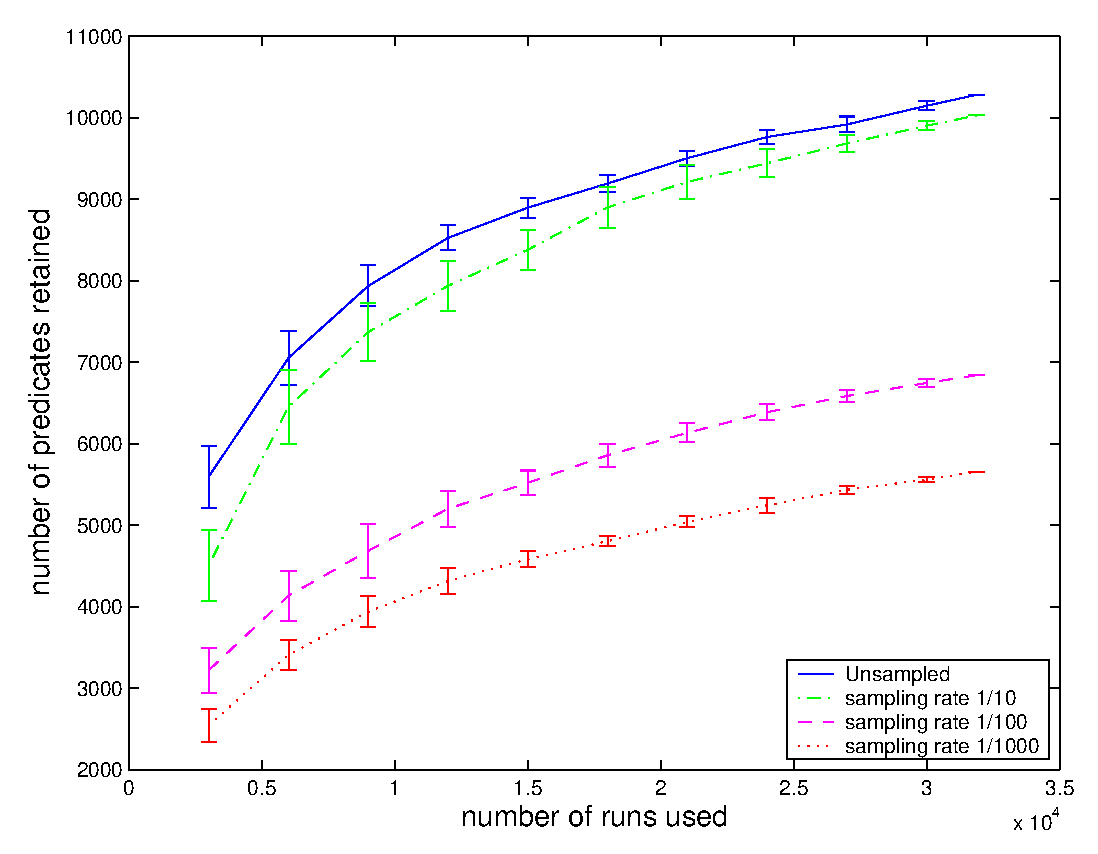
\includegraphics[width=\columnwidth]{predkept3a}\label{fig:predkept-a}}
  \hfill
  \subfigureautorefname[branches and returns only]{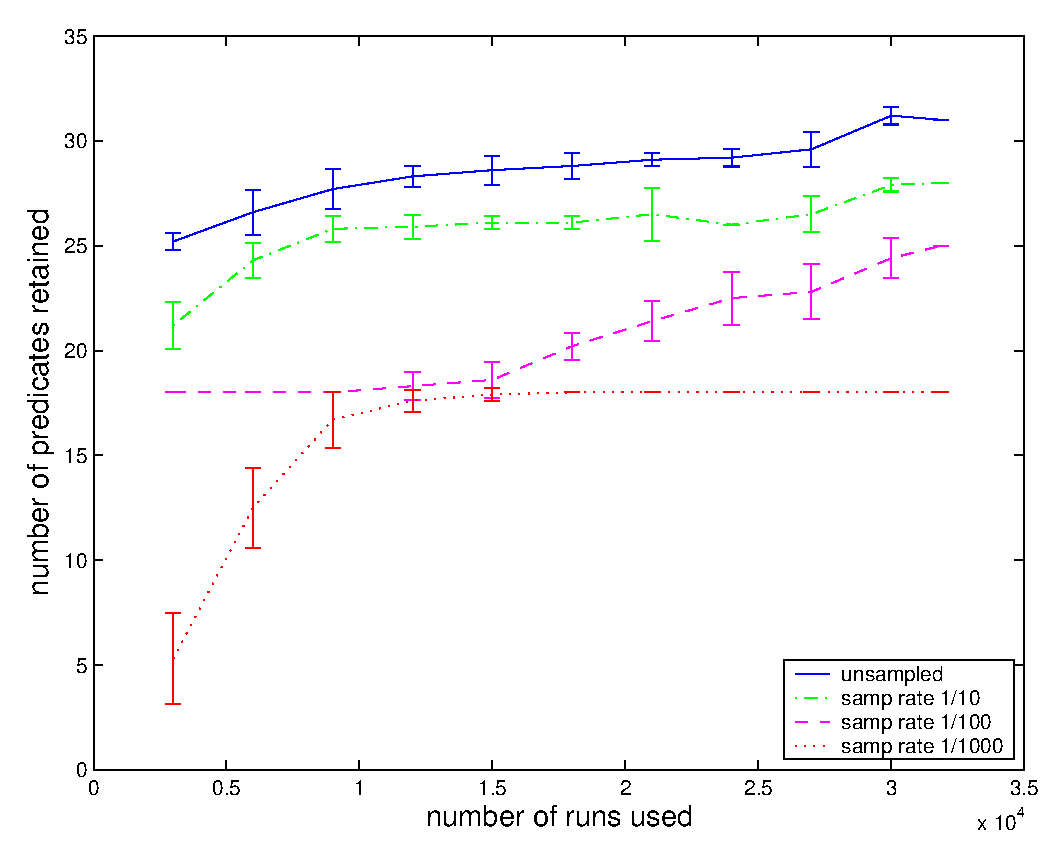
\includegraphics[width=\columnwidth]{predkept3b}\label{fig:predkept-b}}

  \caption{The effect of sampling and data size on the number of
  predicates selected.}\label{fig:predkept}
\end{figure*}

Two trends are apparent from \Autoref{fig:predkept}.  As one would expect,
the number of retained predicates decreases as the sampling rate decreases,
and increases as more trial runs are included.  If we had an unlimited number
of trial runs, the number of retained predicates at all sampling rates should
approach the result with no sampling.  

Note also that increasing 
the number of trial runs always seems to increase the number of retained 
scalar-pairs predicates, whereas the branch and returns predicates run into 
a plateau at lower sampling rates.  Though there may not be much significance 
in this discovery, we conjecture that it is due to the fact that scalar
pairs predicates are much more often observed than the other two kinds of
predicates.  Therefore determining the importance of scalar pairs predicates
takes much fewer sampled trial runs.

%% As is apparent from the graph, there is much larger variation in the
%% number of selected predicates when we use fewer trial runs.
%% %Using $3000$ trials, at the minimum we
%% %retain $7429$ predicates using unsampled data, $7654$ when sampling
%% %rate is $\nicefrac{1}{10}$, $7347$ at $\nicefrac{1}{100}$, and $6750$
%% %at $\nicefrac{1}{1000}$;
%% As we incorporate more examples of successful and failed \moss\ runs,
%% the variances decrease for all sampling rates, but the means behave
%% somewhat differently.  When the data is not sampled, the average
%% number of selected predicates stays around $8100$ for all data sizes.
%% Sampling adds noise to this procedure.  As we observed previously,
%% a moderate sampling rate tends to drive up the $\increase(\ldots)$ scores, and
%% thus enlarges our set of selected predicates (except when we are using
%% very few trial runs).

%% At the relatively high sampling rate of
%% \nicefrac{1}{10}, there are still enough samples taken at most
%% instrumentation sites, and there is a net increase in the number of
%% selected predicates.  Once the sampling rate shrinks to
%% \nicefrac{1}{100} and below, however, the effect of sparse
%% sampling sets in.  Fewer samples are taken overall on fewer predicates,
%% and as a result, fewer predicates have a nonzero $\increase(\ldots)$ score.
%% Incorporating more runs tends to alleviate the situation; at above
%% 10,000 runs, roughly the same number of predicates are retained for
%% the \nicefrac{1}{100} sampled data as the complete data.  The very
%% sparse sampling rate of \nicefrac{1}{1000}, on the other hand,
%% causes much more change in the final result.  A lot more predicates
%% are eliminated when using fewer trials, and a lot more predicates are
%% retained using more trials.

%% Most of the volatility in the results come from the scalar-pair
%% predicates.  \Autoref{fig:predkept-b} shows the same graph for
%% only the branch and return predicates.  Here, across all data sizes,
%% the number of selected predicates remains roughly constant at each
%% sampling rate.  The complete data is still able to select the fewest
%% number of predicates, with \nicefrac{1}{100} sampled data following
%% close behind.  The \nicefrac{1}{1000} sampled data still produces a
%% net increase in the number of selected predicates.

%% LocalWords:  downsampling lang downsampled predelim predkept



\section{Related Work}
\label{sec:related-work}

In this section we briefly survey related work.
The Daikon project \cite{ernst2001} monitors instrumented applications
to discover likely program invariants.  It collects extensive trace
information at run time and uses this offline to accept or reject any
of a wide variety of guessed candidate predicates.  The DIDUCE project
\cite{ICSE02*291} tests a more restricted set of predicates within the
client program, and attempts to relate state changes in candidate
predicates to manifestation of bugs.  Both projects assume complete
monitoring, such as within a controlled test environment.  Our goal is
to use lightweight partial monitoring, suitable for deployment to end
users.  We never have complete information, and therefore must use a
more statistical approach.

\termdef{Software tomography} as realized through the GAMMA system
\cite{PASTE'02*2,Orso:2003:LFDIART} shares our goal of low-overhead
distributed monitoring of deployed code.  GAMMA collects code coverage
data to support a variety of code evolution tasks.  Our
instrumentation exposes a broader family of data- and
control-dependent predicates on program behavior and uses randomized
sparse sampling to control overhead.  We observe, however, that the
predicates injected by our instrumentor can approximate coverage: over
many runs, the sum of all predicate counters at a site converges on
the relative coverage of that site.

Efforts to directly apply statistical modeling principles to debugging
have met with mixed results.  Early work in this area by Burnell and
Horvitz \cite{Burnell:1995:SCM} uses program slicing in conjunction
with Bayesian belief networks to filter and rank the possible causes
for a given bug.  Empirical evaluation shows that the slicing component
alone finds 65\% of bug causes, while the probabilistic model
correctly identifies another 10\%.  This additional payoff may seem
small in light of the effort, measured in multiple
man-years, required to distill experts' often tacit knowledge into a
formal belief network.  However, the approach does illustrate one
strategy for integrating information about program structure into the
statistical modeling process.

In more recent work, Podgurski et al.\ \cite{ICSE`03*465} apply
statistical feature selection, clustering, and multivariate
visualization techniques to the task of classifying software failure
reports.  The intent is to bucket each report into an equivalence
group believed to share the same underlying cause.  Features are
derived offline from fine-grained execution traces without sampling;
this reduces the noise level of the data but greatly restricts the
instrumentation schemes that are practical to deploy outside of a
controlled testing environment.  As in our own earlier work, Podgurski
uses logistic regression to select features which are highly
predictive of failure.  
Clustering tends to identify small, tight groups of runs which do
share a single cause but which are not always maximal.  That is, one
cause may be split across several clusters.

In contrast, current
industrial practice uses stack traces to cluster failure reports into
equivalence classes.  Two crash reports showing the same stack trace,
or perhaps only the same top-of-stack function, are presumed to be two
reports of the same failure.  This works to the extent that a single
cause corresponds to a single point of failure, but our experience
with \moss suggests that this assumption may not often hold.  We find
that only bugs \#2 and \#5 have truly unique ``signature'' stacks: a
crash location which is present if and only if the corresponding bug
was actually triggered.  These bugs are also our most deterministic.
Bugs \#4 and \#6 have nearly unique stack signatures, modulo small
changes to frames several levels removed from the point of failure.
The remaining bugs are much less consistent: each stack signature is
observed after a variety of different bugs, and each triggered bug
causes failure in a variety of different stack states.  Stack-based
clustering provides little insight for temporally extended bugs that
do not crash until well after the bad behavior.  A special case of
this is a program which produces incorrect output but exits normally
without crashing and therefore without any crash stack on which to
cluster.

Studies that attempt real-world deployment of monitored software must
address a host of practical engineering concerns, from distribution to
installation to user support to data collection and warehousing.
Elbaum and Hardojo \cite{Elbaum:2003:DISATA} have reported on a
limited deployment of instrumented Pine binaries.  Their experiences
have helped to guide our own design of a wide public deployment of
applications with sampled instrumentation, presently underway
\cite{Liblit:2003:CBIP}.

For some highly available systems, even a single failure must be
avoided.  Once the behaviors that predict imminent failure are known,
automatic corrective measures may be able to prevent the failure from
occurring at all.  The Software Dependability Framework (SDF)
\cite{Gross:2003:PSMUST} uses the multivariate state estimation
technique to model and thereby predict impending system failures.
Instrumentation is assumed to be complete and is typically
domain-specific, whereas our sampled predicates cast a wider, less
specialized net.

\section{Conclusions and Future Work}
\label{sec:conclusions}

We have demonstrated a practical algorithm for isolating multiple bugs
in complex software systems.  Given feedback profiles of enough runs,
overall trends emerge which can help to guide an engineer to the most
likely causes of the most common bugs.  Our approach uses lightweight,
sampled instrumentation suitable for wide scale deployment to real end
users, which means that the system also performs implicit triage: it
learns the most, most quickly, about the bugs that happen most often.
The key property of our approach is that it filters potential causes
based on the degree to which they increase the likelihood of failure.
Our algorithm appears to do a good job of isolating a wide variety of
bugs, even when multiple bugs are present simultaneously.

When hunting for bugs, the first thing an engineer wants to know is
under what circumstances the failure occurs.  Perhaps the most salient
feature of our approach is the ability to pinpoint the circumstances
under which bugs occur.

We also see several possible avenues for improvement, which we leave
as future work:
\begin{itemize}

\item The scalar-pairs instrumentation scheme induces many
predicates and finds fewer bugs than the branches and
returns instrumentation schemes.  A more specialized version of scalar-pairs
would be useful.

\item To date, we have sampled all sites at the same rate.  However,
rarely executed code, such as code that executes once on system start-up,
can be sampled at a higher rate with no impact on overall performance.
Moreover, infrequently executed code is more likely
to harbor bugs.  By observing rare events more often, we would need fewer
runs to isolate bugs.

\item The algorithm we present here analyzes every predicate independently
of every other predicate.  While we have not yet found a statistical algorithm that exploits
correlations between predicates effectively in the presence of
multiple bugs, we believe this is a worthwhile direction
to explore.
\end{itemize}


\bibliography{cacm1990,icse02,icse03,misc,paste02,pldi03,pods,ramss,refs}

\end{document}

%% LocalWords:  DIDUCE Burnell Horvitz Podgurski Elbaum Hardojo SDF
%% LocalWords:  topcrash cacm icse ramss pldi Podgurski's Kanduri
%% LocalWords:  McMaster Umranov Votta
